\subsection{Lake-at-Rest Over an Uncertain Bed}

This test assesses the ability of the well-balanced stochastic Galerkin models to preserve the C-property for a lake at rest over an uncertain bed.
An analytic solution of the test preserves the quiescent state forever, but numerical methods that are not well-balanced can produce spurious flows.

To present a more challenging test, a rectangular obstacle is introduced to the right of the uncertain hump, so the bed elevation $z$ becomes
\begin{subequations}
\begin{align}
    z(x, a) &= a \sech^2 \left( \frac{\pi x}{\lambda} \right) + \zstar(x) \text{,} \\
    \zstar(x) &= \begin{cases}
    \amean & \text{if $30 < x \leq 40$,} \\
    0 & \text{otherwise}
    \end{cases}
\end{align}
\end{subequations}

Using the $\eta$-form model, a lake-at-rest is easily constructed by choosing initial conditions with zero mean discharge and a uniform mean water elevation $\eta_0 = \SI{1.5}{\meter}$.
To preserve the C-property, second and higher moments of the flow are set to zero so that the initial flow has no uncertainty.

Using the $h$-form model, the initial water height must be specified rather than the initial water elevation.
Since the bed elevation has a region of uncertainty, it is not obvious how a balanced initial condition should be specified to obtain uniform initial water elevation with zero uncertainty.
Instead, an initial condition is specified with uniform mean water height $h_0 = \SI{1.5}{\meter}$ with second and higher moments of the flow set to zero, and the $h$-form model is allowed to find its own balanced state over time.

To assess the well-balancedness of the $\eta$-form and $h$-form stochastic models, results are compared with those of a stochastic model having a centred difference approximation of the bed slope source term that is not well-balanced.
The centred difference model is the same as the well-balanced $\eta$-form model except that the stochastic bed slope source term is
\begin{align}
    \Ensemble{\source_i \pcbasis_l} =
    \left[ 0, -g \sum_{p=0}^P \sum_{q=0}^P \eta_{i,p}
    \frac{z_{i+1,q} - z_{i-1,q}}{2 \Delta x}
    \Ensemble{\pcbasis_p \pcbasis_q \pcbasis_l} \right]^\T
\end{align}

\begin{figure}
\centering
\centering
\begin{subfigure}{\textwidth}
\phantomsubcaption\label{fig:lakeatrest:centred:eta}
\phantomsubcaption\label{fig:lakeatrest:hform:eta}
\phantomsubcaption\label{fig:lakeatrest:etaform:eta}
\phantomsubcaption\label{fig:lakeatrest:centred:q}
\phantomsubcaption\label{fig:lakeatrest:hform:q}
\phantomsubcaption\label{fig:lakeatrest:etaform:q}
\centering
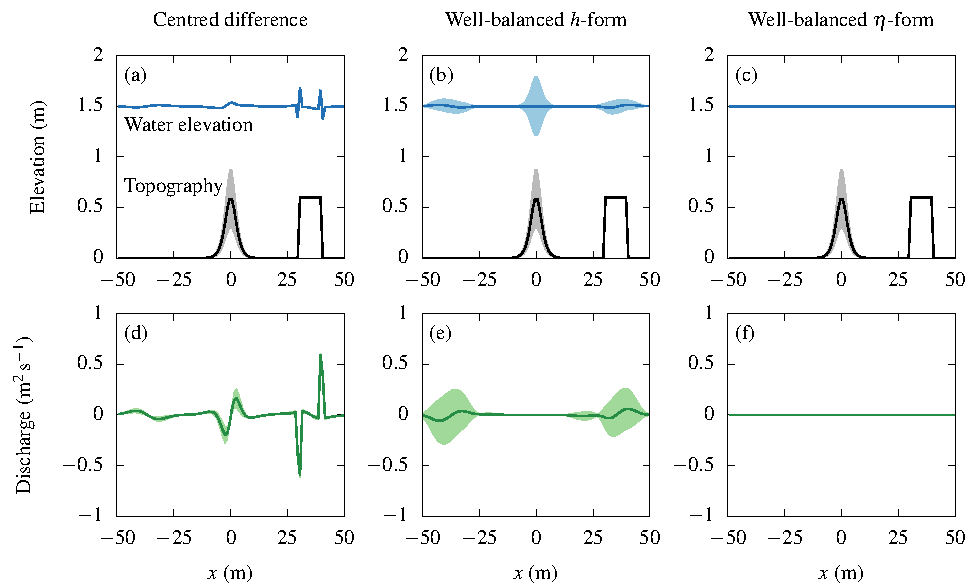
\includegraphics{fig-lakeatrest.pdf}
\end{subfigure}
\caption{Stochastic lake-at-rest solutions at $t = \SI{10}{\second}$.  Mean values are marked by solid lines and shaded regions represent one standard deviation.}
\label{fig:lakeatrest}
\end{figure}

The bed elevation, water elevation and discharge profiles at $t = \SI{10}{\second}$ for the three stochastic Galerkin models are shown in figure~\ref{fig:lakeatrest}.
The lack of well-balancing is apparent using the centred difference model: grid-scale standing waves develop at the discontinuities either side of the rectangular hump (figure~\ref{fig:lakeatrest:centred:eta}, \ref{fig:lakeatrest:centred:q}), and a smooth standing wave also develops over the topographic hump.  These errors persist throughout the simulation.

Using the well-balanced $h$-form model, the mean water elevation is calculated as $\mu_1[\eta] = h_0 + z_0$, and the standard deviation is plotted relative to this mean (figure~\ref{fig:lakeatrest:hform:eta}).
The $h$-form model is initialised in an unbalanced state, and waves are generated over the uncertain topography that propagate away in both directions.  After $t = \SI{10}{\second}$, these waves reach the domain boundaries (figure~\ref{fig:lakeatrest:hform:eta}, figure~\ref{fig:lakeatrest:hform:q}) and exit the domain shortly afterwards.
\todo[inline]{Except for these waves, the mean water elevation is uniformly \SI{1.5}{\meter} (or thereabouts!).
The standard deviation in water height around the hump is equal to the the prescribed standard deviation in bed elevation.  This makes sense because lower topography would result in higher water and vice versa.
Once the model reaches a balanced state, the coefficient $h_1 = - z_1$ and $h_p = 0$ for $p > 1$.
$z$ and $h$ are, in effect, directly correlated.
We chose to plot the standard deviation in water height relative to the mean water elevation.  If we had plotted relative to $\mu_1[\eta] \pm \sqrt{\mu_2[z]}$ then there would be no blue shading in the figure~\ref{fig:lakeatrest:hform:eta} and it we would see that the $h$-form model is indeed well-balanced.
}

\begin{itemize}
    \item when water elevation is lowered to \SI{1.1}{\meter} then the well-balanced $\eta$-form model crashes.  The same problem occurs as the stochastic polynomial degree $P$ is increased.
    This is a known problem with classical Weiner-Hermite \citep{pettersson2014}: with increasingly high-order in random space, the quadrature points in the flux integration get further into the tails of the Gaussian distribution, which can lead to negative water heights being provided as input to the Riemann solver.
\end{itemize}
